%%%%%%%%%%%%%%%%%%%%%%%%%%%%%%%%%%%%%%%%%%%%%%%%%%%%%%%%%%%%%%%%%%%%%%%%%%%%%%%%
%2345678901234567890123456789012345678901234567890123456789012345678901234567890
%        1         2         3         4         5         6         7         8

%\documentclass[letterpaper, 10 pt, conference]{ieeeconf}  % Comment this line out
                                                          % if you need a4paper
\documentclass[letterpaper, 10pt, conference]{ieeeconf}      % Use this line for a4
                                                          % paper

 
\IEEEoverridecommandlockouts                              % This command is only
                                                          % needed if you want to
                                                          % use the \thanks command
\overrideIEEEmargins
% See the \addtolength command later in the file to balance the column lengths
% on the last page of the document

\usepackage{amsmath}    % need for sub equations
\usepackage{amsfonts}
\usepackage{graphicx}   % need for figures
\usepackage{subcaption}
\usepackage{epsfig} 
\usepackage{cancel}
\usepackage{amssymb}
\usepackage{color}
\usepackage[ruled,vlined,titlenotnumbered]{algorithm2e} 

\newcommand{\R}{\mathbb{R}}
\newcommand{\cset}{\mathcal{U}}
\newcommand{\cfset}{\mathbb{U}}
\newcommand{\dfset}{\mathbb{D}}
\newcommand{\dset}{\mathcal{D}}
\newcommand{\obsset}{\mathcal{G}} % Obstacle (the one used to solve PDE)
\newcommand{\ioset}{\mathcal{O}} % Induced obstacle
\newcommand{\brs}{\mathcal{V}} % backwards reachable set
\newcommand{\frs}{\mathcal{W}} % forwards reachable set
\newcommand{\pfrs}{\mathcal{P}} % projected forwards reachable set
\newcommand{\targetset}{\mathcal{T}}
\newcommand{\edt}{t_0}
\newcommand{\sta}{t_\text{STA}}
\newcommand{\dz}{\mathcal{A}} % Avoid set
\newcommand{\cradius}{R_c} % Capture radius
\newcommand{\pos}{p} % position
\newcommand{\npos}{h} % non-position states
\newcommand{\veh}{Q} % vehicle
\newcommand{\dist}{\text{dist}} % Distance
\newcommand{\rc}{R_c} % Capture radius

\title{\LARGE \bf
Safe Sequential Path Planning of Multi-Vehicle Systems Under Presence of Disturbances and Measurement Noise}

\author{Somil Bansal*, Mo Chen*, Jaime F. Fisac, and Claire J. Tomlin
\thanks{This work has been supported in part by NSF under CPS:ActionWebs (CNS-931843), by ONR under the HUNT (N0014-08-0696) and SMARTS (N00014-09-1-1051) MURIs and by grant N00014-12-1-0609, by AFOSR under the CHASE MURI (FA9550-10-1-0567). The research of M. Chen and J. F. Fisac have received funding from the ``NSERC'' program and ``la Caixa" Foundation, respectively.}
\thanks{* Both authors contributed equally to this work. All authors are with the Department of Electrical Engineering and Computer Sciences, University of California, Berkeley. \{mochen72, somil, jfisac, tomlin\}@eecs.berkeley.edu}
}

\begin{document}
\maketitle
\thispagestyle{empty}
\pagestyle{empty}

%%%
\begin{abstract}
\end{abstract}

% !TEX root = ../SPP_IoTjournal.tex
\section{Introduction \label{sec:introduction}}
Recently, there has been an immense surge of interest in the use of unmanned aerial systems (UASs) for civil applications. The applications include package delivery, aerial surveillance, disaster response, among many others \cite{Tice91, Debusk10, Amazon16, AUVSI16, BBC16}. These civil applications will involve unmanned aerial vehicles (UAVs) flying in urban environments, potentially in close proximity to humans, other UAVs, and other important assets. As a result, government agencies such as the Federal Aviation Administration (FAA) and National Aeronautics and Space Administration (NASA) of the United States are urgently trying to develop new scalable ways to organize an airspace in which potentially thousands of UAVs can fly together \cite{FAA13, Kopardekar16}.

One essential problem that needs to be addressed for this endeavor to be successful is that of trajectory planning: how a group of vehicles in the same vicinity can reach their destinations while avoiding situations which are considered dangerous, such as collisions. Many previous studies address this problem under different assumptions. In some studies, specific control strategies for the vehicles are assumed, and approaches such as those involving induced velocity obstacles \cite{Fiorini98, Chasparis05, Vandenberg08,Wu2012} and involving virtual potential fields to maintain collision avoidance \cite{Olfati-Saber2002, Chuang07} have been used. Methods have also been proposed for real-time trajectory generation \cite{Feng-LiLian2002}, for path planning for vehicles with linear dynamics in the presence of obstacles with known motion \cite{Ahmadzadeh2009}, and for cooperative path planning via waypoints which do not account for vehicle dynamics \cite{Bellingham}. Other related work is in the collision avoidance problem without path planning. These results include those that assume the system has a linear model \cite{Beard2003, Schouwenaars2004, Stipanovic2007}, rely on a linearization of the system model \cite{Massink2001, Althoff2011}, assume a simple positional state space \cite{Lin2015}, and many others \cite{Lalish2008, Hoffmann2008, Chen2016}.

However, to make sure that a dense group of UAVs can safely fly in close vicinity of each other, we need the capability to flexibly plan provably safe and dynamically feasible trajectories without making strong assumptions on the vehicles' dynamics and other vehicles' motion. Moreover, any trajectory planning scheme that addresses collision avoidance must also guarantee both goal satisfaction and safety of UAVs despite disturbances caused by wind and communication faults \cite{Kopardekar16}. Furthermore, unexpected scenarios such as UAV malfunctions or even UAVs with malicious intent need to be accounted for. Finally, the proposed scheme should scale well with the number of vehicles.

The problem of trajectory planning and collision avoidance under disturbances in safety-critical systems has been studied using Hamilton-Jacobi (HJ) reachability analysis, which provides guarantees on goal satisfaction and safety of optimal system trajectories \cite{Barron90, Mitchell05, Bokanowski10, Bokanowski11, Margellos11, Fisac15}. Reachability-based methods are particularly suitable in the context of UAVs because of the formal guarantees that are provided. In reachability analysis, one computes the reach-avoid set, defined as the set of states from which the system can be driven to a target set while satisfying time-varying state constraints at all times. A major practical appeal of this approach stems from the availability of modern numerical tools, which can compute various definitions of reachable sets \cite{Sethian96, Osher02, Mitchell02, Mitchell07b}. These numerical tools, for example, have been successfully used to solve a variety of differential games, trajectory planning problems, and optimal control problems. Concrete practical applications include aircraft auto-landing \cite{Bayen07}, automated aerial refueling \cite{Ding08}, MPC control of quadrotors \cite{Bouffard12}, and multiplayer reach-avoid games \cite{Huang11}. Despite its power, the approach becomes numerically intractable as the state space dimension increases. In particular, reachable set computations involve solving a HJ partial differential equation (PDE) or variational inequality (VI) on a grid representing a discretization of the state space, resulting in an \textit{exponential} scaling of computational complexity with respect to the dimensionality of the problem. Therefore, as such, dynamic programming-based approaches such as reachability analysis are not suitable for managing the next generation airspace, which is a large-scale system with a high-dimensional joint state space because of the possible high density of vehicles that needs to be accommodated \cite{Kopardekar16}.  

To overcome this problem, the Sequential Path Planning (SPP) method has been proposed \cite{Chen15c}, in which vehicles are assigned a strict priority ordering. Higher-priority vehicles plan their trajectories without taking into account the lower-priority vehicles. Lower-priority vehicles treat higher-priority vehicles as moving obstacles. Under this assumption, time-varying formulations of reachability \cite{Bokanowski11, Fisac15} can be used to obtain the optimal and provably safe trajectories for each vehicle, starting from the highest-priority vehicle. Thus, the curse of dimensionality is overcome for the multi-vehicle trajectory planning problem at the cost of a structural assumption, under which the computation complexity scales just \textit{linearly} with the number of vehicles. In addition, a structure like this has the potential to flexibly divide up the airspace for the use of many UAVs and allows a tractable multi-vehicle trajectory-planning. In general, different economic mechanisms can be used to come up with a priority order. One example could be first-come-first-serve mechanism, as highlighted in NASA’s concept of operations for UAS traffic management \cite{Kopardekar16}. \SBnote{Mo, could you please read this paragraph again?}

The authors in \cite{Bansal2017} extend the SPP method to the scenarios where disturbances, such as wind, are present in the system, resolving some of the practical challenges associated with the basic SPP algorithm in \cite{Chen15c}. However, if a vehicle not in the set of SPP vehicles enters the system, or even worse, if this vehicle has malicious intent, the original plan can lead to vehicles entering into another vehicle’s danger zone. Thus, if vehicles do not plan with an additional safety margin that takes a potential intruder into account, a vehicle trying to avoid the intruder may effectively become an intruder itself, leading to a domino effect, causing the entire SPP structure to collapse. 

The authors in \cite{chen2016robust} propose an SPP algorithm that accounts for such a potential intruder. However, a new full-scale trajectory planning problem is required to be solved in real time to ensure safe transit of the vehicles to their respective destinations. Since the replanning must be done in real-time, the proposed algorithm is intractable for large-scale systems even with the SPP structure, rendering the method unsuitable for practical implementation in these cases. In this work, we propose a novel intruder avoidance algorithm, which will need to replan trajectories only for a \textit{fixed number of vehicles} if the intruder appears in the system, irrespective of the total number of SPP vehicles. Moreover, this number is a design parameter, which can be chosen beforehand based on the computational resources available for replanning during the run time, thus overcoming the limitations of the algorithm in \cite{chen2016robust}. 

Intuitively, for every vehicle, we compute a \textit{separation region} such that the vehicle needs to account for the intruder if and only if the intruder is inside this separation region. We then compute a \textit{buffer region} between the separation regions of any two vehicles, and ensure that this buffer is maintained as vehicles are traveling to their destinations. Thus, to intrude with any additional vehicle, the intruder will have to travel through this buffer region. In fact, we can affect this traveling time based on the size of the buffer region. Thus, for a given time duration, we can design the buffer region size such that the intruder can affect atmost a desirable number of vehicles. A high-level overview of the proposed algorithm is provided in Algorithm \ref{alg:basic_idea}.    
%
\begin{algorithm}[tb]
\SetKwInOut{Input}{input}
\SetKwInOut{Output}{output}
	\DontPrintSemicolon
	\caption{Overview of the proposed intruder avoidance algorithm (planning phase)}
	\label{alg:basic_idea}
	\Input{Set of vehicles $\veh_i, i = 1, \ldots, \N$ in the descending priority order;\newline
	Vehicle dynamics and initial states;\newline
	Vehicle destinations and any obstacles to avoid;\newline
	Intruder dynamics;\newline
	$\nva$: Maximum number of vehicles allowed to re-plan their trajectories.}
    \Output{Provably safe vehicle trajectories to respective destinations despite disturbance and intruder;\newline 
    Intruder avoidance and goal-satisfaction controller.}
	\For{\text{$i=1:N$}}{
			compute the separation region of $\veh_i$;\;
			compute the required buffer region based on $\nva$;\;
			use SPP algorithm for trajectory planning of $\veh_i$ such that the buffer region is maintained between $\veh_i$ and $\veh_j$ for all $j<i$;\;
			output the trajectory and optimal controller for $\veh_i$.\;
		}
\end{algorithm}
%

The rest of the paper is organized as follows: in Section \ref{sec:formulation}, we formally present the SPP problem in the presence of disturbances and adversarial intruders. In Section \ref{sec:background}, we present a brief review of time-varying reachability and the basic SPP algorithms proposed in \cite{Chen15c}, \cite{Bansal2017}. In Section \ref{sec:intruder}, we explain the proposed algorithm to account for intruders. Finally, we illustrate this algorithm through a fifty-vehicle simulation in an urban environment in Section \ref{sec:simulations}. All running notations in this paper are summarized in Table \ref{table:notation}.
% Introduction (1-1.5p)
%% Motivation
%% Related work
%% Summary of results

% !TEX root = ../SPP_IoTjournal.tex
\section{Sequential Path Planning Problem \label{sec:formulation}}
Consider $\N$ vehicles $\veh_i, i = 1, \ldots, \N$ (also denoted as \textit{SPP vehicles}) which participate in the SPP process. We assume their dynamics are given by

\begin{equation}
\label{eq:dyn}
\begin{aligned}
\dot\state_i &= \fdyn_i(\state_i, \ctrl_i, \dstb_i), t \le \sta_i \\
\ctrl_i &\in \cset_i, \dstb_i \in \dset_i, i = 1 \ldots, \N
\end{aligned}
\end{equation}

\noindent where $\state_i \in \R^{n_i}$, $\ctrl_i \in \cset_i$ and $\dstb_i \in \dset_i$, respectively, represent the state, control and disturbance experienced by vehicle $\veh_i$. We partition the state $\state_i$ into the position component $\pos_i \in \R^{n_\pos}$ and the non-position component $\npos_i \in \R^{n_i - n_\pos}$: $\state_i = (\pos_i, \npos_i)$. %We assume that the control functions $\ctrl_i(\cdot), \dstb_i(\cdot)$ are drawn from the set of measurable functions\footnote{A function $f:X\to Y$ between two measurable spaces $(X,\Sigma_X)$ and $(Y,\Sigma_Y)$ is said to be measurable if the preimage of a measurable set in $Y$ is a measurable set in $X$, that is: $\forall V\in\Sigma_Y, f^{-1}(V)\in\Sigma_X$, with $\Sigma_X,\Sigma_Y$ $\sigma$-algebras on $X$,$Y$.}. For convenience, 
We will use the sets $\cfset_i, \dfset_i$ to respectively denote the set of functions from which the control and disturbance functions $\ctrl_i(\cdot), \dstb_i(\cdot)$ are drawn.

% We further assume that the flow field $\fdyn_i: \R^{n_i}\times\cset_i\times\dset_i \rightarrow \R^{n_i}$ is uniformly continuous, bounded, and Lipschitz continuous in $\state_i$ for fixed $\ctrl_i$ and $\dstb_i$. With this assumption, given $\ctrl_i(\cdot) \in \cfset_i, \dstb_i(\cdot) \in \dfset_i$, there exists a unique trajectory solving \eqref{eq:dyn} \cite{EarlA.Coddington1955}. %We will denote trajectories of \eqref{eq:dyn} starting from state $\state^0_i$ at time $t_0$ under control $\ctrl_i(\cdot)$ and disturbance $\dstb_i(\cdot)$ as $\traj_i(t; \state^0_i, t_0, \ctrl_i(\cdot))$. Trajectories satisfy an initial condition and the differential equation \eqref{eq:dyn} almost everywhere:

%\begin{equation}
%\begin{aligned}
%\frac{d}{dt}\traj_i(t; \state^0_i, t_0, \ctrl_i(\cdot)) &= \fdyn(\state^0_i, \ctrl_i, \dstb_i) \\
%\traj_i(t_0; \state^0_i, t_0, \ctrl_i(\cdot)) &= \state^0_i
%\end{aligned}
%\end{equation}

%In addition, we assume that the disturbances $\dstb_i(\cdot)$ are drawn the set of non-anticipative strategies \cite{Mitchell05} $\Gamma$, defined as follows:
%\begin{equation}
%\begin{aligned}
%& \Gamma := \{\mathcal{N}: \cfset_i \rightarrow \dfset_i:  \ctrl_i(r) = \hat{\ctrl}_i(r) \text{ a. e. } r\in[t,s] \\
%& \Rightarrow \mathcal{N}[\ctrl_i](r) = \mathcal{N}[\hat{\ctrl}_i](r) \text{ a. e. } r\in[t,s]\}
%\end{aligned}
%\end{equation}

Each vehicle $\veh_i$ has initial state $\state^0_i$, and aims to reach its target $\targetset_i$ by some scheduled time of arrival $\sta_i$. The target in general represents some set of desirable states, for example the destination of $\veh_i$. %For most of the paper we will make the assumption that $\edt_i$ is early enough for $\veh_i$ to feasibly get to $\targetset_i$ on time; this can be done by letting $\edt_i \rightarrow -\infty$. The assumption on $\edt_i$ is merely for convenience: in situations where $\edt_i$ is $-\infty$. In some situations, we may find that it is infeasible for $\veh_i$ to get to $\targetset_i$ at or before $\sta_i$. Whenever unsure, we may first determine the earliest feasible $\sta_i$ as described in Section \ref{sec:intruder}.
On its way to $\targetset_i$, $\veh_i$ must avoid a set of static obstacles $\soset_i \subset \R^{n_i}$. The interpretation of $\soset_i$ could be any set of states that are forbidden for each SPP vehicle such as a tall building. Each vehicle $\veh_i$ must also avoid the danger zones with respect to every other vehicle $\veh_j, j\neq i$. The danger zones in general can represent any joint configurations between $\veh_i$ and $\veh_j$ that are considered to be unsafe. We define the danger zone of $\veh_i$ with respect to $\veh_j$ to be
\begin{equation} \label{eqn:danger_zone_defn}
\dz_{ij} = \{(\state_i, \state_j): \|\pos_i - \pos_j\|_2 \le \rc\}
\end{equation}
\noindent whose interpretation is that $\veh_i$ and $\veh_j$ are considered to be in an unsafe configuration when they are within a distance of $\rc$ of each other. In particular, $\veh_i$ and $\veh_j$ are said to have collided, if $(\state_i, \state_j) \in \dz_{ij}$.

In addition to the obstacles and danger zones, an intruder vehicle can also appear in the system. An intruder vehicle may have malicious intent or it can be a non-participating vehicle, which does not have malicious intent, but can accidentally cause a collision with other vehicles since it may not follow the SPP structure. This general definition of intruder allows us to develop algorithms that can also account for vehicles who are not communicating with the SPP vehicles or do not know about the SPP structure. \SBnote{Mo, could you please read this paragraph again? Also, do you think we should expand on this idea of ``non-participating" vehicles in the introduction?}

In general, the effect of an intruder on the vehicles in structured flight can be entirely unpredictable, since the intruder in principle could be adversarial in nature, and the number of intruders could be arbitrary. In particular, if the number of intruders in the system is arbitrary, a collision avoidance problem must to be solved for each SPP vehicle in the joint state-space of all intruders and the vehicle, even with the SPP structure. Therefore, to make our analysis intractable, we make the following two assumptions: \SBnote{Mo, could you please read this paragraph again?}
\begin{assumption}
\label{as:avoidOnce}
At most one intruder (denoted as $\veh_I$ here on) affects the SPP vehicles at any given time. The intruder is removed after a duration of $\iat$. 
\end{assumption}    
This assumption can be valid in situations where intruders are rare, and that some fail-safe or enforcement mechanism exists to force the intruder out of the planning space affecting the SPP vehicles. For example, when SPP vehicles are flying at a particular altitude level, the removal of the intruder can be achieved by exiting the altitude level.
 
Let the time at which intruder appears in the system be $\tsa$ and the time at which it disappears be $\tea$. Assumption \ref{as:avoidOnce} implies that $\tea \leq \tsa + \iat$. Thus, any vehicle $\veh_i$ would need to avoid the intruder $\veh_{\intr}$ for a maximum duration of $\iat$. After a duration of $\iat$, the intruder is no longer present in the system. Note that we do not pose any restriction on $\tsa$; we only assume that once the intruder appears, it stays for a maximum duration of $\iat$.
\begin{assumption}
\label{as:dynKnown}
The dynamics of the intruder are known and given by $\dot\state_\intr = f_\intr(\state_\intr, \ctrl_\intr, \dstb_\intr)$.
\end{assumption}
Assumption \ref{as:dynKnown} is required for HJ reachability analysis. In situations where the dynamics of the intruder are not known exactly, a conservative model of the intruder may be used instead. We also denote the initial state of the intruder as $\state_{\intr}^0.$ Note that $\state_{\intr}^0$ is unknown.

Given the set of SPP vehicles, their targets $\targetset_i$, the static obstacles $\soset_i$, the vehicles' danger zones with respect to each other $\dz_{ij}$, and the intruder dynamics $f_\intr(\cdot)$, our goal is as follows. For each vehicle $\veh_i$, synthesize a controller which guarantees that $\veh_i$ reaches its target $\targetset_i$ at or before the scheduled time of arrival $\sta_i$, while avoiding the static obstacles $\soset_i$, the danger zones with respect to all other vehicles $\dz_{ij}, j\neq i$, and the intruder vehicle $\veh_{\intr}$, irrespective of the control strategy of the intruder. In addition, we would like to obtain the latest departure time $\ldt_i$ such that $\veh_i$ can still arrive at $\targetset_i$ on time.

In general, the above optimal path planning problem must be solved in the joint space of all $\N$ SPP vehicles and the intruder vehicle. However, due to the high joint dimensionality, a direct dynamic programming-based solution is intractable. Therefore, the authors in \cite{Chen15c} proposed to assign a priority to each vehicle, and perform SPP given the assigned priorities. Without loss of generality, let $\veh_j$ have a higher priority than $\veh_i$ if $j<i$. Under the SPP scheme, higher-priority vehicles can ignore the presence of lower-priority vehicles, and perform path planning without taking into account the lower-priority vehicles' danger zones. A lower-priority vehicle $\veh_i$, on the other hand, must ensure that it does not enter the danger zones of the higher-priority vehicles $\veh_j, j<i$ or the intruder vehicle $\veh_{\intr}$; each higher-priority vehicle $\veh_j$ induces a set of time-varying obstacles $\ioset_i^j(t)$, which represents the possible states of $\veh_i$ such that a collision between $\veh_i$ and $\veh_j$ or $\veh_i$ and $\veh_{\intr}$ could occur.

It is straight-forward to see that if each vehicle $\veh_i$ is able to plan a trajectory that takes it to $\targetset_i$ while avoiding the static obstacles $\soset_i$, the danger zones of \textit{higher-priority vehicles} $\veh_j, j<i$, and the danger zone of the \textit{intruder} $\veh_{\intr}$ irrespective of the intruder's control policy, then the set of SPP vehicles $\veh_i, i=1,\ldots,\N$ would all be able to reach their targets safely. Under the SPP scheme, path planning can be done sequentially in descending order of vehicle priority in the state space of only a single vehicle. Thus, SPP provides a solution whose complexity scales linearly with the number of vehicles, as opposed to exponentially, with a direct application of dynamic programming approaches. 

However, when an intruder appears in the system, depending on the initial state of the intruder and its control policy, a vehicle may arrive at different states after avoiding the intruder. Therefore, a control policy that ensures a successful transit to the destination needs to account for all such possible states, which is a path planning problem with multiple initial states and a single destination, and is hard to solve in general. Thus, we divide the intruder avoidance problem into two sub-problems: (i) we first design a control policy that ensures a successful transit to the destination if no intruder appears and that successfully avoid the intruder, if it does (Algorithm \ref{alg:basic_idea}). (ii) after the intruder disappears at $\tea$, we replan the trajectories of the affected vehicles. Following the same theme and assumptions, the authors in \cite{chen2016robust} present an algorithm to avoid an intruder in SPP formulation; however, in the worst-case, the algorithm might need to replan the trajectories for \textit{all} SPP vehicles. Since the replanning is done in real-time, the method in \cite{chen2016robust} is unsuitable for practical implementation for large multi-vehicle systems. Our goal in this work is to present an algorithm that ensures that only a \textit{small and fixed} number of vehicles need to replan their trajectories, regardless of the total number of vehicles. Thus, the replanning time is constant and can be done in real time. In particular, we answer the following inter-dependent questions:
\begin{enumerate}
\item How can each vehicle guarantee that it will reach its target set without getting into any danger zones, despite no knowledge of the intruder initial state, the time at which it appears, and its control strategy?
\item How can we ensure that replanning only needs to be done for at most a fixed maximum number of vehicles after the intruder disappears from the system? \label{question2}
\item Can we choose the maximum number of the vehicles in question \ref{question2} above?
\end{enumerate}

\begin{table*}
    \caption{Different mathematical notations and their interpretation (in the alphabetical order of symbols).}    
    \resizebox{\hsize}{!}{
    \begin{tabular}{ |>{\centering\arraybackslash}m{1.5cm}| m{5cm} | m{3cm} | m{\columnwidth} |}
 %   \begin{tabular}{ | l | l | p{11cm} |}
    \hline
    \textbf{Notation} & \textbf{Description} & \textbf{Location} & \textbf{Interpretation} \\ \hline
    
    %%% Letter D %%% 
    % Disturbance
    $\dstb_i$ & Disturbance in the dynamics of vehicle $i$ & Beginning of Section \ref{sec:formulation} & -    \\ \hline   
    $\dstb_{\intr}$ & Disturbance in the dynamics of the intruder & Assumption \ref{as:dynKnown} & -    \\ \hline   
    
    %%% Letter F %%%
    % Dynamics
    $\fdyn_i$ & Dynamics of vehicle $i$ & Beginning of Section \ref{sec:formulation} & -    \\ \hline
    $f_\intr$ & Dynamics of the intruder & Assumption \ref{as:dynKnown} & -    \\ \hline
    $f_r$ & Relatiove dynamics between two vehicles & Equation \eqref{eq:reldyn} & - \\ \hline
    
    %%% Letter G %%%
    % Obstacle
    $\obsset_i(t)$ & The overall obstacle for vehicle $i$ & Equation \eqref{eq:obsseti} & The set of states that vehicle $i$ must avoid on its way to the destination. \\ \hline
    
    %%% Letter H %%%
    % Non-position state components of the vehicle
    $\npos_i$ & Non-position state component of vehicle $i$ & Beginning of Section \ref{sec:formulation} & -    \\ \hline
    
    %%% Letter K %%%
    % Number of vehicles to avoid
    $\nva$ & - & Beginning of Section \ref{sec:intruder} & The maximum number of vehicles that should apply the avoidnace maneuver or the maximum number of vehicles that we can replan trajectories for in real-time.    \\ \hline    
    
    %%% Letter L %%%
    % Target set
    $\targetset_i$ & Target set of vehicle $i$ & Beginning of Section \ref{sec:formulation} & The destination of vehicle $i$.    \\ \hline
    
    %%% Letter M %%%    
    % Base obstacles
    $\boset_j(t)$ & Base obstacle induced by vehicle $j$ at time $t$ & Equations (25), (31) and (37) in \cite{chen2016robust} & The set of all possible states that vehicle $j$ can be in at time $t$ if the intruder does not appear in the system till time $t$. \\ \hline    
    
    %%% Letter N %%%
    % Number of vehicles
    $\N$ & Number of SPP vehicles & Beginning of Section \ref{sec:formulation} & -    \\ \hline
    
    %%% Letter O %%%
    % Obstacles
	$\ioset_i^j(t)$ & Induced obstacle by vehicle $j$ for vehicle $i$ & After Assumption \ref{as:dynKnown} in Section \ref{sec:formulation} & The possible states of vehicle $i$ such that a collision between vehicle $i$ and vehicle $j$ or vehicle $i$ and the intruder vehicle (if present) could occur.    \\ \hline 
	% Static Obstacles   
    $\soset_i$ & Static obstacle for vehicle $i$ & Beginning of Section \ref{sec:formulation} & Obstacles that vehicle $i$ needs to avoid on its way to destination, e.g, tall buildings. \\ \hline    
    
    %%% Letter P %%%
    % Position state components of the vehicle
    $\pos_i$ & Position of vehicle $i$ & Beginning of Section \ref{sec:formulation} & -    \\ \hline
     
    %%% Letter Q %%%
    % SPP vehicle
    $\veh_{i}$ & $i$th SPP vehicle & Beginning of Section \ref{sec:formulation} & -  \\ \hline
    % Intruder vehicle
    $\veh_{\intr}$ & The intruder vehicle & Assumption \ref{as:avoidOnce} & -  \\ \hline
    
    %%% Letter R %%%
    % Unsafe distance
    $\rc$ & Danger zone radius & Equation \eqref{eqn:danger_zone_defn} & The closest distance between vehicle $i$ and vehicle $j$ that is considered to be safe. \\ \hline  
    
    %%% Letter S %%%
    % Separation Region
    $\sep_j(t)$ & Separation region of vehicle $j$ at time $t$ & Beginning of Section \ref{sec:sepRegion_case1} & The set of all states of intruder at time $t$ for which vehicle $j$ is forced to apply an avoidance maneuver. \\ \hline        
    
    %%% Letter T %%%
    % Avoid start time
    $\tsa_i$ & Avoid start time of vehicle $i$ & Equation \eqref{eqn:avoidStartTime2} & The first time at which vehicle $i$ is forced to apply an avoidance maneuver by the intruder vehicle. Defined to be $\infty$ if vehicle $i$ never applies an avoidance maneuver.\\ \hline    
    % Buffer region duration
    $\brd$ & Buffer region travel duration & Beginning of Section \ref{sec:intruder} & The minimum time required for the intruder to travel through the buffer region between any pair of vehicles. \\ \hline
    % Intruder avoidance time
    $\iat$ & Intruder avoidance time & Assumption \ref{as:avoidOnce} & The maximum duration for which the intruder is present in the system. \\ \hline
    % Intruder appearance time
    $\tsa$ & Intruder appearance time & After Assumption \ref{as:avoidOnce} & The time at which the intruder appears in the system. \\ \hline
    % Intruder avoidance time
    $\tea$ & Intruder disappearance time & After Assumption \ref{as:avoidOnce} & The time at which the intruder disappears from the system. \\ \hline
    % Latest Departure Time
    $\ldt_i$ & Latest departure time of vehicle $i$ & End of Section \ref{sec:formulation} & The latest departure time for vehicle $i$ such that it safely reaches its destination by the scheduled time of arrival. \\ \hline
    % Scheduled time of arrival
    $\sta_i$ & Scheduled time of arrival (STA) of vehicle $i$ & Beginning of Section \ref{sec:formulation} & The time by which vehicle $i$ is required to reach its destination.    \\ \hline
    
 
	%%% Letter U %%% 
    % control
    $\ctrl_i$ & Control of vehicle $i$ & Beginning of Section \ref{sec:formulation} & -    \\ \hline   
    $\ctrl_{\intr}$ & Control of the intruder & Assumption \ref{as:dynKnown} & -    \\ \hline    
    ${\ctrl^{\text{A}}_{i}}$ & Optimal avoidance control of vehicle $i$ & Equation \eqref{eqn:optAvoidCtrl} & The control that vehicle $i$ need to apply to successfully avoid the intruder once the relative state between vehicle $i$ and the intruder reaches the boundary of the avoid region of vehicle $i$.  \\ \hline    

    %%% Letter V %%%
    % Avoid region
    $\brs^{\text{A}}_{i}(\tau, \iat)$ & Avoid region of vehicle $i$ & Equation \eqref{eqn:avoidBRS} & The set of relative states $\state_{\intr i}$ for which the intruder can force vehicle $i$ to enter in the danger zone $\dz_{i \intr}$ within a duration of $(\iat-\tau)$. \\ \hline

 	%%% Letter X %%%    
    % State of the vehicle
    $\state_i$ & State of vehicle $i$ & Beginning of Section \ref{sec:formulation} & - \\ \hline
    % State of the intruder
    $\state_{\intr}$ & State of the intruder vehicle & Assumption \ref{as:dynKnown} & - \\ \hline
    % State of the vehicle
    $\state_i^0$ & Initial state of vehicle $i$ & Beginning of Section \ref{sec:formulation} & - \\ \hline
    % State of the intruder
    $\state_{\intr}^0$ & Initial state of the intruder vehicle & Assumption \ref{as:dynKnown} & - \\ \hline
    % Relative State
    $\state_{\intr i}$ & Relative state between the intruder and vehicle $i$ & Equation \eqref{eq:reldyn} & - \\ \hline
    
   
    %%% Letter Z %%%    
    % Danger Zone
    $\dz_{ij}$ & Danger zone between vehicle $i$ and vehicle $j$ & Equation \eqref{eqn:danger_zone_defn} & Set of all states of vehicle $i$ and vehicle $j$ which are within unsafe distance of each other. The vehicles are said to have collided if their states belong to $\dz_{ij}$. \\ \hline
    
    \end{tabular}
    }
    \label{table:notation}
\end{table*}


% Problem formulation (1.5p)
%% A number of aircrafts aiming to reach a number of destinations respectively, on a certain schedule
%% Disturbance
%% How to guarantee they all get there and on time?
%% Feedback control (centralized server) or distributed control (naive forward reachable set)

% !TEX root = SPP2.tex
\section{Solution via double-obstacle HJI VI and SPP\label{sec:solution}}
\subsection{Double-Obstacle Hamilton-Jacobi Variational Inequality}
Our solution method takes advantage of the double-obstacle HJ approach \cite{Fisac15}, in which one computes the reachable set $\brs(t)$ in the presence of a time-varying target set $\targetset(t)$ and time-varying obstacles $\obsset(t)$. Mathematically, we are given a system with state $z$ evolving according to

\begin{equation}
\label{eq:fdyn} % Full dynamics
\begin{aligned}
\dot{z} &= f(t, z, u, d), \quad t \in [0, T] \\
z(0) &= z_0, \quad u \in \cset, d \in \dset
\end{aligned}
\end{equation}

After defining some target set $\targetset(t)$, we compute the backwards reachable set $\brs(t)$, defined by
%
\begin{equation}
\label{eq:brs}
\begin{aligned}
&\brs(t) = \{z: \exists u \in \cfset, \forall \gamma[u] \in \Gamma, \eqref{eq:fdyn} \\
&\Rightarrow \exists s \in [t, T], z(s) \in \targetset(s) \wedge z(\tau) \notin \obsset(\tau) \forall \tau \in [t, s]\}
\end{aligned}
\end{equation}
%
\noindent where $\cfset$ is the set of measurable functions satisfying control constraints at every $t$, and $\Gamma$ is the set of nonanticipative strategies \cite{Mitchell05} defined as follows \MCnote{Check notation!}:

\begin{equation}
\begin{aligned}
\gamma &\in \Gamma := \{\mathcal{N}: \mathbb{U}_1 \rightarrow \mathbb{U}_2 \mid  u_1(r) = \hat{u}_1(r) \\
&\text{for almost every } r\in[t,s] \Rightarrow \mathcal{N}[u_1](r) \\
&= \mathcal{N}[\hat{u}_1](r) \text{ for almost every } r\in[t,s]\}
\end{aligned}
\end{equation}

Intuitively, the reachable set is the set of states from which exists a control such that for all non-anticipative disturbances, the system is driven into the target set $\targetset(t)$ in the time horizon $[t, T]$ without first entering the obstacle set $\obsset(t)$.

Given the target set $\targetset(t)$ specified as an implicit surface function such that $\targetset(t) = \{z: l(t, z) \le 0\}$, the reachable set can be obtained as the implicit surface function such that $\brs(t) = \{z: V(t, z) \le 0\}$, where $V(t, z)$ is the viscosity solution \cite{Crandall83} to the following HJ variational inequality:
%
\begin{equation}
\label{eq:HJIVI}
\begin{aligned}
\max\Big\{&\min\big\{D_t V(t, z) + H\left(t, z, D_z V\right), l(t,z) - V(t, z)\big\}\\
& -g(t, z) - V(t, z)\Big\} = 0, \quad t\in[0,T]\\
&V(T, x) = \max\big\{l(T, x), -g(T, x)\big\} \\
&H\left(t, z, p\right) = \min_{u \in \cset} \max_{d \in \dset} p \cdot f(t, z, u, d)
\end{aligned}
\end{equation}
%
\noindent where $g(t, x)$ is the implicit surface function representing $\obsset(t)$: $\obsset(t) = \{z: g(t, x) \le 0\}$. After the reachable set is computed, the optimal control can be obtained as follows:
%
\begin{equation}
\label{eq:opt_ctrl}
u^*(t, z) = \arg \min_{u \in \cset} \max_{d \in \dset} H\left(t, z, D_z V\right)
\end{equation}

In theory, one could define the state to be the joint states of all vehicles, $z = (x_1, x_2, \ldots, x_N)$, define the dynamics \eqref{eq:fdyn} to follow $\eqref{eq:dyn}$, the target set $\targetset$ to correspond to the situation in which all vehicles have arrived at their targets $\targetset_i, i = 1, \ldots, N$, and the obstacle set $\obsset$ to correspond to the union of all the danger zones $\dz_{ij}$. Then, \eqref{eq:HJIVI} could be solved to obtain $\brs(t)$, and then the joint optimal control would be given by \eqref{eq:opt_ctrl}.

However, practically, the dimensionality of the joint state $z$ would be extremely high. In fact, for even the simplest vehicle models, solving \eqref{eq:HJIVI} would be intractable for more than two vehicles. Therefore, we propose the sequential path planning method, which allows \eqref{eq:HJIVI} to be solved in the state space of each vehicle, making the computation complexity scale linearly, as opposed to exponentially, with the number of vehicles.

\subsection{Sequential Path Planning}
In order to make the $N$-vehicle path planning problem safe and tractable, we impose a slight structure to the problem: each vehicle is assigned a priority. When planning its trajectory to its target, a higher priority vehicle can disregard the presence of a lower priority vehicle. In contrast, a lower priority vehicle must take into account the presence of all higher priority vehicles, and plan its trajectory in a way that avoids the higher priority vehicles' danger zones. For convenience, denote the vehicle with the $i$th highest priority as $\veh_i$.

Optimal path planning in this setting is enabled by the HJ variational inequality which computes the backwards reachable set $\brs_i$ from a target set $\targetset_i$ in the presence of time-varying obstacles $\obsset_i$. In the sequential path planning application, the time-varying obstacles represent regions of the state space of $\veh_i$ that must be avoided in order to ensure that $\veh_i$ does not enter any danger zones of higher priority vehicles. We present three different ways to compute $\obsset_i$, obstacles induced by higher priority vehicles in Section \ref{sec:obs_gen}. For now, we proceed assuming $\obsset_i$ is given.

To obtain the optimal control for to reach the target we adapt \eqref{eq:HJIVI} to $\veh_i$ and solve the following PDE:
%
\begin{equation}
\label{eq:HJIVI_i}
\begin{aligned}
\max\Big\{&\min\big\{D_t V_i(t, x_i) + H_i\left(t, x_i, D_{x_i} V\right),\\
& l_i(t, x_i) - V_i(t, x_i)\big\}, -g_i(t, x_i) - V_i(t, x_i)\Big\} = 0, \\
& t \in [\edt, \sta]\\
&V_i(\sta, x_i) = \max\big\{l_i(x_i), -g_i(\sta, x_i)\big\} \\
&H_i\left(t, x_i, p\right) = \min_{u_i \in \cset_i} \max_{d_i \in \dset_i} p \cdot f(t, x_i, u_i, d_i)
\end{aligned}
\end{equation}

Here, the target set $\targetset_i$, obstacle set $\obsset_i(t)$, and backwards reachable set $\brs_i(t)$ are related to $l_i(x_i), g_i(t, x_i), V_i(t, x_i)$ as follows:
%
\begin{equation}
\begin{aligned}
\targetset_i &= \{x_i: l_i(x_i) \le 0\} \\
\obsset_i(t) &= \{x_i: g_i(t, x_i) \le 0\} \\
\brs_i(t) &= \{x_i: V_i(t, x_i) \le 0\}
\end{aligned}
\end{equation}

From the reachable set, the optimal control for vehicle $\veh_i$ is then given as
\begin{equation}
\label{eq:opt_ctrl_i}
u_i^*(t, x_i) = \arg \min_{u_i \in \cset_i} H_i\left(t, x_i, D_{x_i} V_i\right)
\end{equation}

If $\veh_i$ uses the optimal control given by \eqref{eq:opt_ctrl_i}, then $\veh_i$ can be guaranteed to reach the target $\targetset_i$ as long as $\veh_i$ departs at the latest departure time $\ldt_i$, defined as $\inf_t V_i(t, x_i) \le 0$.
% Solution methodology (1.5-2.5p)
%% Variational inequality to be solved
%% Backwards reachability

% Obstacle generation
% !TEX root = ../SPP_journal.tex
\section{SPP With Disturbances and Incomplete Information \label{sec:incomp}}
Disturbances and incomplete information significantly complicate the SPP scheme. The main difference is that the vehicle dynamics satisfy \eqref{eq:dyn} as opposed to \eqref{eq:dyn_no_dstb}. Committing to exact trajectories is therefore no longer possible, since the disturbance $\dstb_i(\cdot)$ is \textit{a priori} unknown. Thus, the induced obstacles $\ioset_i^j(t)$ are no longer just the danger zones centered around positions. 

\subsection{Theory}
We present three methods to address the above issues. The methods differ in terms of control policy information that is known to a lower-priority vehicle, and have their relative advantages and disadvantages depending on the situation. The three methods are as follows:
\begin{itemize}
\item \textbf{Centralized control}: A specific control strategy is enforced upon a vehicle; this can be achieved, for example, by some central agent such as an air traffic controller.
\item \textbf{Least restrictive control}: A vehicle is required to arrive at its target on time, but has no other restrictions on its control policy. When the control policy of a vehicle is unknown, but its timely arrive at its target can be assumed, the least restrictive control can be safely assumed by lower-priority vehicles.
\item \textbf{Robust trajectory tracking}: A vehicle declares a nominal trajectory which can be robustly tracked under disturbances.
\end{itemize}

In general, the above methods can be used in combination in a single path planning problem, with each vehicle independently having different control policies. Lower-priority vehicles would then plan their paths while taking into account the control policy information known for each higher-priority vehicle. For clarity, we will present each method as if all vehicles are using the same method of path planning.

In addition, for simplicity of explanation, we will assume that no static obstacles exist. In the situations where static obstacles do exist, the time-varying obstacles $\obsset_i(t)$ simply become the union of the induced obstacles $\ioset_i^j(t)$ in \eqref{eq:ioset} and the static obstacles. The material in this section is taken partially from \cite{Bansal2017}.

\subsubsection{Centralized Control\label{sec:cc}}
The highest-priority vehicle $\veh_1$ first plans its path by computing the BRS (with $i=1$)
\begin{equation}
\label{eq:BRS}
\begin{aligned}
\brs_i^\text{dstb}(t, \sta_i) = & \{y: \exists \ctrl_i(\cdot) \in \cfset_i, \forall \dstb_i(\cdot) \in \dfset_i, \state_i(\cdot) \text{ satisfies \eqref{eq:dyn}},\\
& \forall s \in [t, \sta_i], \state_i(s) \notin \obsset_i(s), \state_i(t) = y\\
& \exists s \in [t, \sta_i], \state_i(s) \in \targetset_i\}
\end{aligned}
\end{equation}

Since we have assumed no static obstacles exist, we have that for $\veh_1, \obsset_1(s)=\emptyset ~ \forall s \le \sta_i$, and thus the above BRS is well-defined. This BRS can be computed by solving the HJ VI \eqref{eq:HJIVI_BRS} with the following Hamiltonian:

\begin{equation}
\ham_i^\text{dstb}\left(\state_i, \costate\right) = \min_{\ctrl_i \in \cset_i} \max_{\dstb_i \in \dset_i} \costate \cdot \fdyn_i(\state_i, \ctrl_i, \dstb_i)
\end{equation}

From the BRS, we can obtain the optimal control

\begin{equation}
\label{eq:opt_ctrl_i}
\ctrl_i^\text{dstb}(t,\state_i) =  \arg \min_{\ctrl_i \in \cset_i} \max_{\dstb_i \in \dset_i} \costate \cdot \fdyn_i(\state_i, \ctrl_i, \dstb_i)
\end{equation}

Here, as well as in the other two methods, the latest departure time $\ldt_i$ is then given by $\arg \sup_t \state_{i}^0 \in \brs_i^\text{dstb}(t, \sta_i)$.

If there is a central agent directly controlling each of the $N$ vehicles, then the control law of each vehicle can be enforced. In this case, lower-priority vehicles can safely assume that higher-priority vehicles are applying the enforced control law. In particular, the optimal controller for getting to the target, $\ctrl^\text{dstb}_i(t, \state_i)$, can be enforced. In this case, the dynamics of each vehicle becomes 

\begin{equation}
\label{eq:dyn_cc}
\begin{aligned}
\dot \state_i &= \fdyn^\text{cc}_i (t, \state_i, \dstb_i) = \fdyn_i(\state_i, \ctrl^\text{dstb}_i(t,\state_i), \dstb_i) \\
\dstb_i &\in \dset_i, \quad i = 1,\ldots, N, \quad t \in [\ldt_i, \sta_i]
\end{aligned}
\end{equation}

\noindent where $\ctrl_i$ no longer appears explicitly in the dynamics.

From the perspective of a lower-priority vehicle $\veh_i$, a higher-priority vehicle $\veh_j, j < i$ induces a time-varying obstacle that represents the positions that could possibly be within the collision radius $\rc$ of $\veh_j$ under the dynamics $\fdyn^\text{cc}_j(t, \state_j, \dstb_j)$. Determining this obstacle involves computing an FRS of $\veh_j$ starting from\footnote{In practice, we define the target set to be a small region around the vehicle's initial state for computational reasons.} $\state_j(\ldt_j) = \state_{j}^0$. The FRS $\frs_j^\text{cc}(\ldt_j, t)$ is defined as follows:

\begin{equation}
\label{eq:FRS1}
\begin{aligned}
\frs_j^\text{cc}(\ldt_j, t) = & \{y: \exists \dstb_j(\cdot) \in \dfset_j, \state_j(\cdot) \text{ satisfies \eqref{eq:dyn_cc}},\\
& \state_j(\ldt_j) = \state_{j}^0, \state_j(t) = y\}.
\end{aligned}
\end{equation}

This FRS can be computed using \eqref{eq:HJIVI_FRS} with the Hamiltonian

\begin{equation}
\ham_j^\text{cc}\left(t, \state_j, \costate\right) = \max_{\dstb_j \in \dset_j} \costate \cdot f^\text{cc}_j(t, \state_j, \dstb_j)
\end{equation}

The FRS $\frs_j^\text{cc}(\ldt_j, t)$ represents the set of possible states at time $t$ of a higher-priority vehicle $\veh_j$ given all possible disturbances $\dstb_j(\cdot)$ and given that $\veh_j$ uses the feedback controller $\ctrl_j^\text{dstb}(t, \state_j)$. In order for a lower-priority vehicle $\veh_i$ to guarantee that it does not go within a distance of $\rc$ to $\veh_j$, $\veh_i$ must stay a distance of at least $\rc$ away from the FRS $\frs_j^\text{cc}(\ldt_j, t)$ for all possible values of the non-position states $\npos_j$. This gives the obstacle induced by a higher-priority vehicle $\veh_j$ for a lower-priority vehicle $\veh_i$ as follows:

\begin{equation} \label{eqn:ccObs}
\ioset_i^j(t) = \{\state_i: \exists y \in \pfrs_j(t), \|\pos_i - y\|_2 \le \rc \}
\end{equation}

\noindent where the set $\pfrs_j(t)$ is the set of states in the FRS $\frs_j^\text{cc}(\ldt_j, t)$ projected onto the states representing position $\pos_j$, and disregarding the non-position dimensions $\npos_j$:

\begin{align} 
\pfrs_j(t) & = \{p_j: \exists \npos_j, (p_j, \npos_j) \in \boset_j(t) \}, \label{eqn:ccObs_help1}\\
\boset_j(t) & = \frs_j^\text{cc}(\ldt_j, t). \label{eqn:ccObs_help2}
\end{align}

Finally, taking the union of the induced obstacles $\ioset_i^j(t)$ as in \eqref{eq:obsseti} gives us the time-varying obstacles $\obsset_i(t)$ needed to define and determine the BRS $\brs_i^\text{dstb}(t, \sta_i)$ in \eqref{eq:BRS}. Repeating this process, all vehicles will be able to plan paths that guarantee the vehicles' timely and safe arrival. The centralized control algorithm can be summarized as follows:
\begin{alg}
\label{alg:cc}
\textbf{Centralized control algorithm}: Given initial conditions $\state_i^0$, vehicle dynamics \eqref{eq:dyn}, target set $\targetset_i$, and static obstacles $\soset_i, i = 1\ldots, \N$, for each $i$,
\begin{enumerate}
\item determine the total obstacle set $\obsset_i(t)$, given in \eqref{eq:obsseti}. In the case $i=1$, $\obsset_i(t) = \soset_i ~ \forall t$;
\item compute the BRS $\brs_i^\text{dstb}(t, \sta_i)$ defined in \eqref{eq:BRS}. The latest departure time $\ldt_i$ is then given by $\arg \sup_t \state^0_i \in \brs_i^\text{dstb}(t, \sta_i)$;
\item compute the optimal control $\ctrl_i^\text{dstb}(t,\state_i)$ corresponding to $\brs_i^\text{dstb}(t, \sta_i)$ given by \eqref{eq:opt_ctrl_i}. Given $\ctrl_i^\text{dstb}(t,\state_i)$, compute the FRS $\frs_i^\text{cc}(\ldt_i, t)$ in \eqref{eq:FRS1};
\item finally, compute the induced obstacles $\ioset_k^i(t)$ for each $k>i$. In the centralized control method, $\ioset_k^i(t)$ is computed using \eqref{eqn:ccObs} where $\pfrs_i(t)$ is given by \eqref{eqn:ccObs_help1}.
\end{enumerate}
\end{alg} % with feedback control
% !TEX root = SPP2.tex
\subsection{Method 2: Least Restrictive Control \label{sec:lrc}}
If there is no centralized controller to enforce the control policy for higher priority vehicles, weaker assumptions must be made by the lower priority vehicles to ensure collision avoidance. One reasonable assumption that a lower priority vehicle can make is that all higher priority vehicles follow the least restrictive control that would take them to their targets. This control would be given by 

\begin{equation}
\label{eq:lrctrl} % least restrictive control
u_j(t, x_j)\in \begin{cases} \{u_j^*(t, x_j) \text{ given by } \eqref{eq:opt_ctrl_i}\} \text{ if } x_j\in \partial \brs_j(t), \\
\cset_i  \text{ otherwise}
\end{cases}
\end{equation}

Such a controller allows each higher priority vehicle to use any controller it desires, except when it is on the boundary of the BRS, $\partial \brs_j$, in which case the optimal control $u_j^*(t, x_j)$ given by \eqref{eq:opt_ctrl_i} must be used to get to the target on time. This assumption is the weakest assumption that could be made by lower priority vehicles given that the higher priority vehicles will get to their targets on time.

Suppose a lower priority vehicle $\veh_i$ assumes that higher priority vehicles $\veh_j, j < i$ use the least restrictive control strategy \eqref{eq:lrctrl}. From the perspective of the lower priority vehicle $\veh_i$, a higher priority vehicle $\veh_j$ could be in any state that is reachable from $\veh_j$'s initial state $x_j(\edt)$ and from which the target $\targetset_j$ can be reached. Mathematically, this is defined by $\veh_j$ is the intersection of the FRS from the initial state $x_j(\edt)$ and the BRS defined in \eqref{eq:brs} from the target set $\targetset_j$, $\brs_j(t) \cap \frs_j(t)$. In this situation, since $\veh_j$ cannot be assumed to be using any particular feedback control, $\frs_j(t)$ is defined in \eqref{eq:frs2} and can also be computed by solving \eqref{eq:FRS_j}.

\SBnote{traj.-based definition}
\begin{equation}
\label{eq:frs2}
\begin{aligned}
&\frs_j(t) = \{y \in \R^{n_j}: \exists u \in \cfset, \exists d \in \dfset, \\
& \quad \dot{x}_j = f_j(x_j, u_j, d_j) \Rightarrow, x_j(t) = y\}
\end{aligned}
\end{equation}

In turn, the obstacle induced by a higher priority $\veh_j$ for a lower priority vehicle $\veh_i$ is as follows:

\begin{equation}
\ioset_i^j(t) = \{x_i: \dist(\pos_i, \pfrs_j(t)) \le \cradius \}
\end{equation}

\noindent where $\pfrs_j(t)$ is given by

\begin{equation}
\pfrs_j(t) = \{p: \exists \npos_j, (p, \npos_j) \in \brs_j(t) \cap \frs_j(t)\}
\end{equation} % with intersection of FRS and BRS
% !TEX root = SPP2.tex
\subsection{Method 3: Robust Tracking of Nominal Trajectories \label{sec:rtt}}
\SBnote{This section is mathematically sound, but we need to reduce the number of jargon words a little bit to make it simpler to understand.}
%A general issue with the above two methods can be the large size of the generated obstacles due to the uncertainty on other vehicles' motion. In order to reduce this uncertainty,
% This approach requires a moderate amount of information sharing between vehicles: higher-priority vehicles need to declare their nominal trajectory, together with an uncertainty region, to all vehicles with lower priority. Lower-priority vehicles will then use these nominal trajectories ``expanded" by the uncertainty regions as time-varying obstacles.
A third way of computing induced obstacles is to have vehicles commit to robustly tracking a feasible nominal trajectory. If a vehicle can be guaranteed to track a trajectory with a bounded error at all times, then this bound can be used to determine the induced obstacle. \SBnote{Let's mention the two phases here.} The planning phase does not make full use of the vehicle's control authority, as some margin is needed to reject unexpected disturbances. Therefore, with this method, planning is done for a reduced control set $\cset^p\subset\cset$ according to Section \ref{sec:solution}.
\SBnote{What does according to Section \ref{sec:solution} mean?}

%The resulting trajectory reference will not utilize the vehicle's full maneuverability; replicating the nominal control is therefore always possible, with additional maneuverability available at execution time to counteract external disturbances and render the error dynamics asymptotically stable.

In this context, robust nonlinear control techniques such as Lyapunov-based methods \cite{Majumdar2013} can be used to compute robust ``funnels" around a concrete nominal trajectory. In this paper, we use reachability to determine the tracking error bound so that the tracking error bound can be determined independently of the nominal trajectory. 

Here, we wish to find a robust control-invariant set in the joint state space of the vehicle and a tracking reference that may ``maneuver" arbitrarily over time, and in the presence of an unknown bounded disturbance. Taking a worst-case approach, the tracking reference can be viewed as a virtual evader vehicle that is optimally avoiding the actual vehicle to enlarge the tracking error. We therefore can model trajectory tracking as a pursuit-evasion game in which the actual vehicle is playing against the coordinated worst-case action of the virtual vehicle and the disturbance. In general, this game will be governed by dynamics of the form:

\SBnote{We need some explanation on what variables mean in the following equations.} 
\begin{equation}
\label{eq:jdyn} % Joint dynamics
\begin{aligned}
\dot{x} &= f(t, x, u, d), \\
\dot{x_r} &=f(t,x_r,u_r,0),\\
u &\in \cset, u_r\in\cset^p, d \in \dset, \\
&t \in [0, T].
\end{aligned}
\end{equation}

\SBnote{The next two sentences should be moved before the "In general, this game ...." sentence.}
Given an error bound $\errorbound(x_{r,i})$ on the tracking error $e=x-x_r$, we define the target set $\targetset$ for this reachability problem to be the set of joint configurations where this bound is violated: $\targetset = \{(x, x_{r,i}): x\not\in\errorbound(x_{r,i})\}$. In this case, the BRS $\brs(t)$ represents the set of states from which the vehicle may be driven to violate the tracking error bounds, outside of $\errorbound(x_{r,i})$.

%In this case the backwards reachable set $\brs(t)$ is defined as:

%\begin{equation}
%\label{eq:brs}
%\begin{aligned}
%&\brs(t) = \{(x,x_r):  \exists \lambda[u] \in \Lambda, \forall u \in \cfset, \eqref{eq:jdyn} \\
%&\Rightarrow \exists s \in [t, T], (x(s),x_r(s)) \in \targetset(s)\},
%\end{aligned}
%\end{equation}

% where $\Lambda$ is the set of nonanticipative strategies from $\cfset$ to $\cfset^p\times \dfset$.

With analogous definitions as those in Section \ref{sec:solution}, $\brs(t)$ can be characterized as the negative region of the solution $V$ to a simpler case of \eqref{eq:HJIVI}:

\begin{equation}
\label{eq:HJIVI_track}
\begin{aligned}
\min\big\{&D_t V(t, z) + H\left(t, z, D_z V\right), l(t,z) - V(t, z)\big\}= 0,\\&  t\in[0,T],\\
&V(T, z) = l(T, z),\\
&H\left(t, z, p\right) = \max_{u \in \cset} \min_{u_r \in\cset^p} \min_{d \in \dset} p \cdot f_z(t,z,u,u_r,d),
\end{aligned}
\end{equation}

\noindent where for compactness of notation we denote $z=(x,x_r)$ and $f_z(t,z,u,u_r,d) = [f(t,x,u,d),f(t,x_r,u_r,0)]$. The complement of $\brs(0)$ is the maximal robust controlled-invariant set in $\targetset^\text{c}$. Letting $T\to\infty$ we obtain the infinite controlled-invariant set, which we denote by $\disckernel$. If this set is nonempty, then the tracking error $e$ at flight time is guaranteed to remain within $\errorbound$ provided that the vehicle starts inside $\disckernel$ and subsequently applies the feedback control law implicitly defined in \eqref{eq:HJIVI_track}:
\begin{equation}\label{eq:robust_tracking_law}
\tracklaw(x,x_r) \in \arg\max_{u \in \cset} \min_{u_r \in\cset^p, d \in \dset} D_z V(0) \cdot f_z(t,z,u,u_r,d).
\end{equation}

In cases where the error dynamics are independent of the absolute state as in \eqref{eq:edyn}, $\disckernel$ can be computed in the state space of the tracking error $e$ to produce a feedback control law that also only depends on $e$, which significantly reduces the problem dimensionality.

\begin{equation}
\label{eq:edyn} % Error dynamics
\begin{aligned}
\dot{e} &= f_e(t, e, u, u_r,d), \\
u &\in \cset, u_r\in\cset^p, d \in \dset, \\
&t \in [0, T],
\end{aligned}
\end{equation}

Given $\errorbound$, we can guarantee that $\veh_i$ will reach its target $\targetset_i$ if $\errorbound \subset \targetset_i$; thus, in the path planning phase, we modify $\targetset_i$ to be $\{x: \errorbound(x) \subseteq \targetset_i\}$.

Finally, since each vehicle $\veh_i$ can only be guaranteed to stay within $\errorbound(x_{r,i})$, we must make sure at any given time, the error bounds of $\veh_i$ and $\veh_j$, $\errorbound(x_{r,i})$ and $\errorbound(x_{r,j})$, do not intersect. This can be done by choosing the induced obstacle to be the Minkowski sum of the error bounds:
\begin{equation}
\ioset_i^j(t) = \errorbound(0) + \errorbound(x_{r,j}(t))
\end{equation}
\SBnote{This equation is a bit confusing. Shouldn't it be $\ioset_i^j(t) = \errorbound(x_{r,i}(t)) + \errorbound(x_{r,j}(t))$?}
\noindent where the $0$ denotes the origin.


%now requiring the state (error) to remain in $\errorbound$, so that the target simply becomes $\targetset = \mathbb{R}^n \setminus \errorbound$. In these cases, \eqref{eq:HJIVI_track} is defined on the lower-dimensional state space of relative (error) dynamics (i.e. over $e$ instead of $z$), and the resulting $\disckernel\subset \mathbb{R}^n$ is the discriminating kernel of $\errorbound$. The flight-time tracking error $e$ is then guaranteed to remain within $\errorbound$ provided that the initial error is contained in $\disckernel$ and the vehicle controller applies the optimally robust tracking feedback law \eqref{eq:robust_tracking_law}, which is now of the form $\tracklaw(e)$.

%A price to be paid for using this method is that it imposes more stringent restrictions on the planning. At flight time, the vehicle will apply this robust tracking law around the nominal trajectory instead of the optimal control policy prescribed by the path planner; while constraint satisfaction is guaranteed for the nominal trajectory, this guarantee does not immediately extend to trajectories within the tracking error bound. The natural solution is to ``robustify" the planning by augmenting all obstacles as $\obsset^\errorbound(t) := \obsset(t) - \errorbound$ (with $-$ denoting the Minkowski difference). It then follows directly that if $x_r(t)$ remains clear of $\obsset^\errorbound(t)$ for all $t$, then $x(t)$ remains clear of the original obstacle $\obsset(t)$.

%Based on this, it will be desirable to choose the tracking error bound $\errorbound$ to be as small as possible. The concrete choice of $\errorbound$ will generally correspond to the system designer, since it is specific to the vehicle dynamics, and should always ensure that the resulting discriminating kernel $\disckernel$ (a) is nonempty and (b) contains all expected errors in the initial configuration. % with bubbles

% !TEX root = ../SPP_IoTjournal.tex
\subsection{Results \label{sec:bayArea_simResults}}
The trajectory planning for the vehicles is done using RTT algorithm, similar to that in Section \ref{sec:city_simResults}. The resulting trajectories of vehicles are shown in Figure \ref{fig:bayArea_d11sep5}. Once again, the vehicles remain clear of all other vehicles and reach their respective destinations. Given the relative separation between the scheduled times of arrival, the trajectories are predominately \textit{time-separated}, with roughly two lanes for each pair of cities (one for going from city A to city B and another for from city B to city A). A high-density of vehicles is achieved in the center since the 4 paths are intersecting in the center (Richmond-Oakland, Oakland-Richmond, Berkeley-San Francisco, San Francisco-Berkeley), but the SPP algorithm ensures safety despite this high-density, as shown in the zoomed-in version of center at an intermediate time when a large number of vehicles are passing through the central region (Figure \ref{fig:bayArea_d11sep5_zoomed}).  
%
\begin{figure*}[!htb]
 \centering
\begin{subfigure}{\columnwidth}
  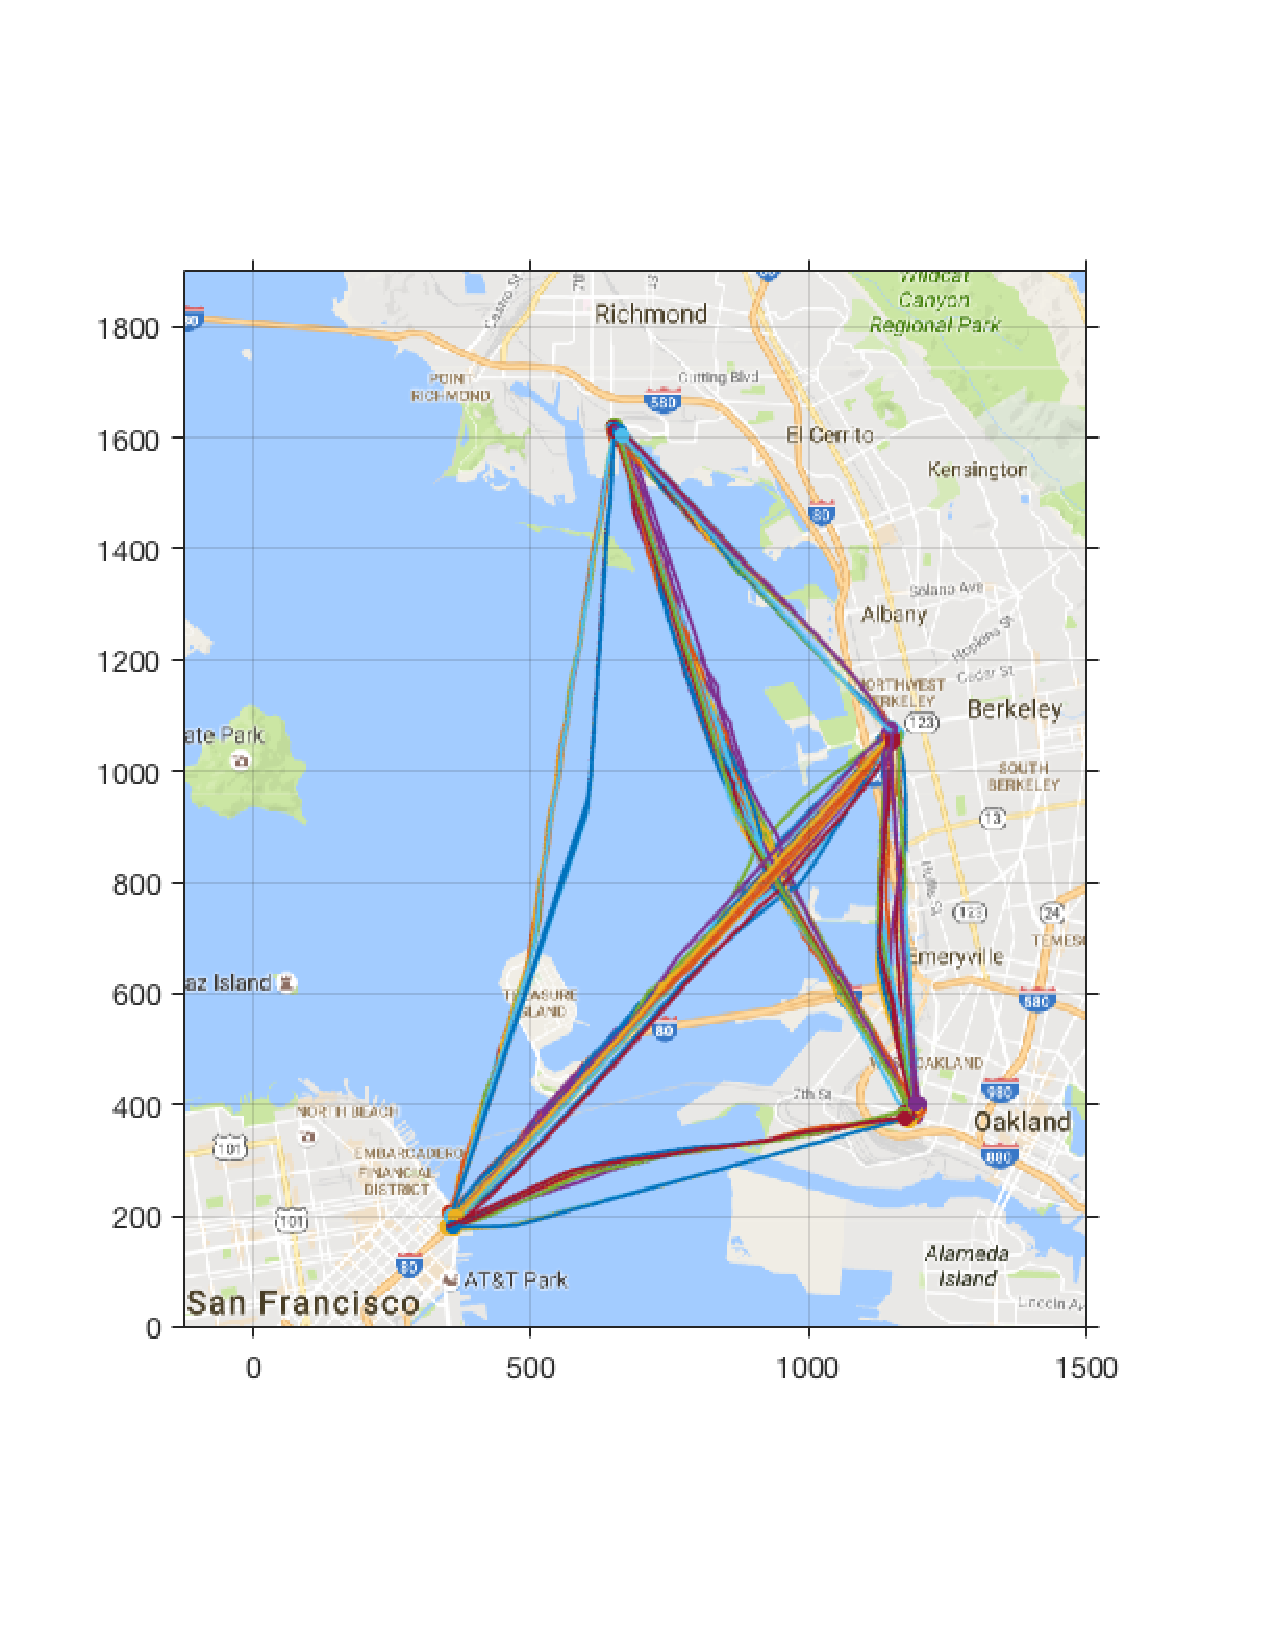
\includegraphics[width=\columnwidth]{figs/bayArea_d11sep5}
  \subcaption{}
  \label{fig:bayArea_d11sep5}
\end{subfigure}%
\begin{subfigure}{\columnwidth}
  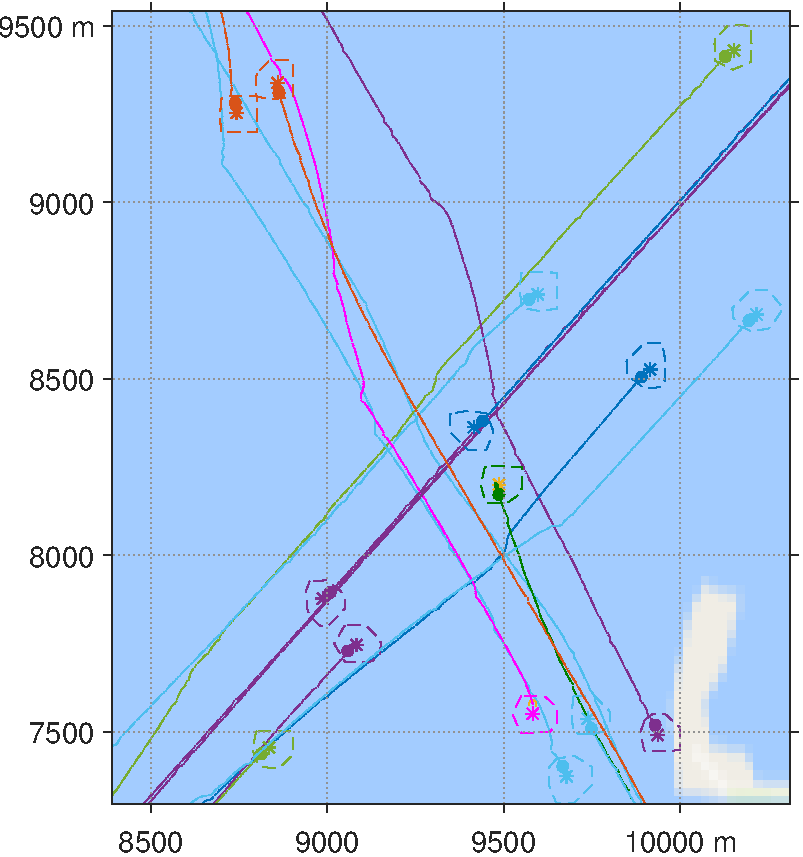
\includegraphics[width=\columnwidth]{figs/bayArea_d11sep5_zoomed}
  \subcaption{}
  \label{fig:bayArea_d11sep5_zoomed}
\end{subfigure}%
  \caption{(a) Trajectories obtained from the SPP algorithm for the multi-city simulation with $d_r = 11m/s$, $\sta_i = 5(i-1)$. (b) Zoomed-in version of the central area. A high density of vehicles is achieved at the center because of the intersection of several trajectories; however, the SPP algorithm still ensures that vehicles do not enter each other's danger zones and reach their destinations.} 
  \label{fig:bayArea_d11sep5_all}
\end{figure*}

Finally, we simulate the system for the case where $\sta_i = 0 ~\forall i$. As evident from Figure \ref{fig:bayArea_d11sep0}, we get multiple lanes between each pair of cities in this case and trajectories become predominately state-separated, as we expect based on the discussion in Section \ref{sec:city_distbEffect}.
\begin{figure}[t]
  \centering
  \includegraphics[width=\columnwidth]{"figs/bayArea_d11sep0"}
  \caption{Vehicle trajectories for $d_r = 11m/s$, $\sta_i = 0$. Since different vehicles have same scheduled times of arrival, a multiple-lane behavior is observed between every pair of cities.} 
  \label{fig:bayArea_d11sep0}
\end{figure}

The average trajectory computation time per vehicle is \SBnote{$XYZ$s} per vehicle on a \SBnote{$Blah Blah$} computing machine. Once again all the computation is done offline and only a lookup table query is required in real-time, which can be performed very efficiently. This simulation illustrates the scalability and the potential of deploying the SPP algorithm for provably safe path planning for large multi-vehicle systems.
% Numerical Simuations (1-2p)

% !TEX root = STP_journal.tex
\section{Conclusions and Future Work}
Guaranteed-safe multi-vehicle trajectory planning is a challenging problem, and previous analyses often either require strong assumptions on the motion of the vehicles or result in a large degree of conservatism. Differential game techniques such as Hamilton-Jacobi (HJ) reachability are ideally suited for guaranteeing goal satisfaction and safety under disturbances, but become intractable for even a small number of vehicles.

Our robust sequential trajectory planning (STP) method assigns a strict priority ordering to vehicles to offer a tractable and practical approach to the multi-vehicle trajectory planning problem. Under the proposed method, a portion of ``space-time'' is reserved for vehicles in the airspace in descending priority order to allow for dense vehicle configurations. Unlike previous priority-based methods, our approach accounts for disturbances and an adversarial intruder. STP reduces the scaling of HJ reachability's computational complexity from exponential to linear with respect to the number of vehicles, while maintaining hard guarantees on goal satisfaction and safety under disturbances. In the presence of a single intruder vehicle, STP still guarantees goal satisfaction and safety with a quadratically scaling computational complexity.

In the future, we plan to investigate ways of guaranteeing a maximum number of vehicles that need to re-plan, combine reachability analysis with other trajectory and path planning methods to improve computation speed, and to better understand the scenarios under which the STP scheme is the most useful by running large-scale simulations.
\vspace{-0.2cm}
% Conclusion (0.5p)

%%%%%%%%%%%%%%%%%%%%%%%%%%%%%%%%%%%%%%%%%%%%%%%%%%%%%%%%%%%%%%%%%%%%%%%%%%%%%%%%
%\addtolength{\textheight}{1cm}   % This command serves to balance the column lengths
                                  % on the last page of the document manually. It shortens
                                  % the textheight of the last page by a suitable amount.
                                  % This command does not take effect until the next page
                                  % so it should come on the page before the last. Make
                                  % sure that you do not shorten the textheight too much.

\bibliographystyle{IEEEtran}
\bibliography{references}
\end{document}
